\def\colegio{Colegio Latinoamericano de Integración}
\def\titulo{Transformaciones isométricas}
\def\subtitulo{La traslación}

\documentclass[]{presentacion}

\NewDocumentCommand{\corazon}{O{0}mm}{
  \addplot [
    samples=100,
    domain=-3:3,
    variable=\t,
    trig format plots=rad,
    rotate around={#1:(#2,#3)}
  ] ( {sin(t)^3 + #2},{(13*cos(t)-5*cos(2*t)-2*cos(3*t)-cos(4*t))/16 + 0.1 + #3} );
}

\NewDocumentCommand{\ticket}{mm}{\node[] at (axis cs: #1,#2) {\check};}
\NewDocumentCommand{\cruz}{mm}{\node[] at (axis cs: #1,#2) {\xmark};}
\ExplSyntaxOn
\NewDocumentCommand{\flecha}{mmmm}{
  \draw[->,shorten~>=0.2cm,shorten~<=0.2cm] (#1,#2) -- (#3,#4)
    node[midway,above,fill=ColorBackground,fill~opacity=1,text~opacity=1,inner~sep=1pt]
      {(\int_eval:n{#3-#1},\int_eval:n{#4-#2})};
}
\ExplSyntaxOff

\begin{document}

\begin{frame}{¿Qué es una traslación?}

\begin{center}
  \begin{tikzpicture}
    \begin{axis}[
        width = .7\linewidth,
        height = .7\linewidth,
        %axis equal,
        grid=major,
        major grid style={gray},
        xmin=0, xmax=10,
        ymin=0, ymax=10,
        xtick distance=1,         % Use tick distance instead of explicit ticks
        ytick distance=1,
        enlarge x limits=false,
        enlarge y limits=false,
        tick align=outside        % Try to align ticks differently
    ]
      \corazon{5}{5}
      \only<2->{\corazon{7}{7}}
      \only<2->{\ticket{7}{7}}
      \only<3->{\flecha{5}{5}{7}{7}}
      \only<4->{\corazon{3}{8}}
      \only<4->{\ticket{3}{8}}
      \only<5->{\flecha{5}{5}{3}{8}}
      \only<6->{\corazon[90]{2}{2}}
      \only<7->{\cruz{2}{2}}
    \end{axis}
  \end{tikzpicture}
\end{center}

\end{frame}

\begin{frame}[allowframebreaks]
\begin{itemize}
  \item askdasdok
  \item askdasdok
  \item askdasdok
  \item askdasdok
  \item askdasdok
  \item askdasdok
  \item askdasdok
  \item askdasdok
  \item askdasdok
  \item askdasdok
  \item askdasdok
  \item askdasdok
  \item askdasdok
  \item askdasdok
  \item askdasdok
  \item askdasdok
  \item askdasdok
  \item askdasdok
  \item askdasdok
  \item askdasdok
  \item askdasdok
  \item askdasdok
  \item askdasdok

\end{itemize}

\end{frame}

\begin{frame}
hola
\begin{ejercicios}(3)
\ejercicio $x^2-3x+1$
\ejercicio $x^2-3x+1$
\ejercicio $x^2-3x+1$
\ejercicio $x^2-3x+1$
\ejercicio $x^2-3x+1$
\ejercicio $x^2-3x+1$
\ejercicio $x^2-3x+1$
\ejercicio $x^2-3x+1$
\ejercicio $x^2-3x+1$
\ejercicio $x^2-3x+1$
\ejercicio $x^2-3x+1$
\end{ejercicios}

\end{frame}

\begin{frame}

\begin{problema}
  some text
\end{problema}

\begin{problema}[1]
  some text
\end{problema}

\begin{problema}[2]
  some text
\end{problema}

\begin{problema}[3]
  some text
\end{problema}

\end{frame}

\end{document}



